\documentclass{ximera}

\usepackage{epsfig}

\graphicspath{
  {./}
  {figures/}
}


\usepackage{morewrites}

%\newcounter{ccounter}
%\setcounter{ccounter}{1}
%\newcommand{\Chapter}[1]{\setcounter{chapter}{\arabic{ccounter}}\chapter{#1}\addtocounter{ccounter}{1}}

%\newcommand{\section}[1]{\section{#1}\setcounter{thm}{0}\setcounter{equation}{0}}

%\renewcommand{\theequation}{\arabic{chapter}.\arabic{section}.\arabic{equation}}
%\renewcommand{\thefigure}{\arabic{chapter}.\arabic{figure}}
%\renewcommand{\thetable}{\arabic{chapter}.\arabic{table}}

%\newcommand{\Sec}[2]{\section{#1}\markright{\arabic{ccounter}.\arabic{section}.#2}\setcounter{equation}{0}\setcounter{thm}{0}\setcounter{figure}{0}}

\newcommand{\Sec}[2]{\section{#1}}

\setcounter{secnumdepth}{2}
%\setcounter{secnumdepth}{1} 

%\newcounter{THM}
%\renewcommand{\theTHM}{\arabic{chapter}.\arabic{section}}

\newcommand{\trademark}{{R\!\!\!\!\!\bigcirc}}
%\newtheorem{exercise}{}

\newcommand{\dfield}{{\sf dfield9}}
\newcommand{\pplane}{{\sf pplane9}}

\newcommand{\EXER}{\section*{Exercises}}%\vspace*{0.2in}\hrule\small\setcounter{exercise}{0}}
\newcommand{\CEXER}{}%\vspace{0.08in}\begin{center}Computer Exercises\end{center}}
\newcommand{\TEXER}{} %\vspace{0.08in}\begin{center}Hand Exercises\end{center}}
\newcommand{\AEXER}{} %\vspace{0.08in}\begin{center}Hand Exercises\end{center}}

% BADBAD: \newcommand{\Bbb}{\bf}

\newcommand{\R}{\mbox{$\Bbb{R}$}}
\newcommand{\C}{\mbox{$\Bbb{C}$}}
\newcommand{\Z}{\mbox{$\Bbb{Z}$}}
\newcommand{\N}{\mbox{$\Bbb{N}$}}
\newcommand{\D}{\mbox{{\bf D}}}
\usepackage{amssymb}
%\newcommand{\qed}{\hfill\mbox{\raggedright$\square$} \vspace{1ex}}
%\newcommand{\proof}{\noindent {\bf Proof:} \hspace{0.1in}}

\newcommand{\setmin}{\;\mbox{--}\;}
\newcommand{\Matlab}{{M\small{AT\-LAB}} }
\newcommand{\Matlabp}{{M\small{AT\-LAB}}}
\newcommand{\computer}{\Matlab Instructions}
\newcommand{\half}{\mbox{$\frac{1}{2}$}}
\newcommand{\compose}{\raisebox{.15ex}{\mbox{{\scriptsize$\circ$}}}}
\newcommand{\AND}{\quad\mbox{and}\quad}
\newcommand{\vect}[2]{\left(\begin{array}{c} #1_1 \\ \vdots \\
 #1_{#2}\end{array}\right)}
\newcommand{\mattwo}[4]{\left(\begin{array}{rr} #1 & #2\\ #3
&#4\end{array}\right)}
\newcommand{\mattwoc}[4]{\left(\begin{array}{cc} #1 & #2\\ #3
&#4\end{array}\right)}
\newcommand{\vectwo}[2]{\left(\begin{array}{r} #1 \\ #2\end{array}\right)}
\newcommand{\vectwoc}[2]{\left(\begin{array}{c} #1 \\ #2\end{array}\right)}



\newcommand{\inv}{^{-1}}
\newcommand{\CC}{{\cal C}}
\newcommand{\CCone}{\CC^1}
\newcommand{\Span}{{\rm span}}
\newcommand{\rank}{{\rm rank}}
\newcommand{\trace}{{\rm tr}}
\newcommand{\RE}{{\rm Re}}
\newcommand{\IM}{{\rm Im}}
\newcommand{\nulls}{{\rm null\;space}}

\newcommand{\dps}{\displaystyle}
\newcommand{\arraystart}{\renewcommand{\arraystretch}{1.8}}
\newcommand{\arrayfinish}{\renewcommand{\arraystretch}{1.2}}
\newcommand{\Start}[1]{\vspace{0.08in}\noindent {\bf Section~\ref{#1}}}
\newcommand{\exer}[1]{\noindent {\bf \ref{#1}}}
\newcommand{\ans}{}
\newcommand{\matthree}[9]{\left(\begin{array}{rrr} #1 & #2 & #3 \\ #4 & #5 & #6
\\ #7 & #8 & #9\end{array}\right)}
\newcommand{\cvectwo}[2]{\left(\begin{array}{c} #1 \\ #2\end{array}\right)}
\newcommand{\cmatthree}[9]{\left(\begin{array}{ccc} #1 & #2 & #3 \\ #4 & #5 &
#6 \\ #7 & #8 & #9\end{array}\right)}
\newcommand{\vecthree}[3]{\left(\begin{array}{r} #1 \\ #2 \\
#3\end{array}\right)}
\newcommand{\cvecthree}[3]{\left(\begin{array}{c} #1 \\ #2 \\
#3\end{array}\right)}
\newcommand{\cmattwo}[4]{\left(\begin{array}{cc} #1 & #2\\ #3
&#4\end{array}\right)}

\newcommand{\Matrix}[1]{\ensuremath{\left(\begin{array}{rrrrrrrrrrrrrrrrrr} #1 \end{array}\right)}}

\newcommand{\Matrixc}[1]{\ensuremath{\left(\begin{array}{cccccccccccc} #1 \end{array}\right)}}



\renewcommand{\labelenumi}{\theenumi)}
\newenvironment{enumeratea}%
{\begingroup
 \renewcommand{\theenumi}{\alph{enumi}}
 \renewcommand{\labelenumi}{(\theenumi)}
 \begin{enumerate}}
 {\end{enumerate}\endgroup}



\newcounter{help}
\renewcommand{\thehelp}{\thesection.\arabic{equation}}

%\newenvironment{equation*}%
%{\renewcommand\endequation{\eqno (\theequation)* $$}%
%   \begin{equation}}%
%   {\end{equation}\renewcommand\endequation{\eqno \@eqnnum
%$$\global\@ignoretrue}}

%\input{psfig.tex}

\author{Martin Golubitsky and Michael Dellnitz}

%\newenvironment{matlabEquation}%
%{\renewcommand\endequation{\eqno (\theequation*) $$}%
%   \begin{equation}}%
%   {\end{equation}\renewcommand\endequation{\eqno \@eqnnum
% $$\global\@ignoretrue}}

\newcommand{\soln}{\textbf{Solution:} }
\newcommand{\exercap}[1]{\centerline{Figure~\ref{#1}}}
\newcommand{\exercaptwo}[1]{\centerline{Figure~\ref{#1}a\hspace{2.1in}
Figure~\ref{#1}b}}
\newcommand{\exercapthree}[1]{\centerline{Figure~\ref{#1}a\hspace{1.2in}
Figure~\ref{#1}b\hspace{1.2in}Figure~\ref{#1}c}}
\newcommand{\para}{\hspace{0.4in}}

\renewenvironment{solution}{\suppress}{\endsuppress}

\ifxake
\newenvironment{matlabEquation}{\begin{equation}}{\end{equation}}
\else
\newenvironment{matlabEquation}%
{\let\oldtheequation\theequation\renewcommand{\theequation}{\oldtheequation*}\begin{equation}}%
  {\end{equation}\let\theequation\oldtheequation}
\fi

\makeatother


\title{The Initial Value Problem}

\begin{document}
\begin{abstract}
\end{abstract}
\maketitle

 \index{initial value problem}
\label{S:6.1}

Recall that a planar autonomous \index{autonomous} constant coefficient system of
ordinary differential equations has the form
\arraystart
\begin{equation}  \label{2dlinsystem}
\begin{array}{ccl}
\dps \frac{dx}{dt}  & = & ax+by \\
\dps \frac{dy}{dt}  & = & cx+dy
\end{array}
\end{equation}
\arrayfinish
where $a,b,c,d\in\R$. Computer experiments using {\pplane} lead us to
believe that there is just one solution to \eqref{2dlinsystem} satisfying
the initial conditions\index{initial condition}
\begin{eqnarray*}
x(0) & = & x_0 \\
y(0) & = & y_0.
\end{eqnarray*}
We prove existence in this section and the next by determining explicit 
formulas for solutions.  

\subsection*{The Initial Value Problem for Linear Systems}
\index{initial value problem}

In this chapter we discuss how to find solutions $(x(t),y(t))$ to
\eqref{2dlinsystem} satisfying the initial values $x(0)=x_0$ and $y(0)=y_0$.
It is convenient to rewrite \eqref{2dlinsystem} in matrix form as:
\begin{equation} \label{ndlinsystem}
\frac{dX}{dt}(t) = CX(t).
\end{equation}
The initial value problem is then stated as:  Find a solution to
\eqref{ndlinsystem} satisfying $X(0)=X_0$ where $X_0=(x_0,y_0)^t$.
Everything that we have said here works equally well for $n$
dimensional systems of linear differential equations.  Just let
$C$ be an $n\times n$ matrix and let $X_0$ be an $n$ vector
of initial conditions.

\subsubsection*{Solving the Initial Value Problem Using Superposition}

In Section~\ref{S:IVPR} we discussed how to solve~\eqref{ndlinsystem} when the
eigenvalues of $C$ are real and distinct.  Recall that when $\lambda_1$ and
$\lambda_2$ are distinct real eigenvalues of $C$ with associated
eigenvectors $v_1$ and $v_2$, there are two solutions to \eqref{ndlinsystem}
given by the explicit formulas
\[
X_1(t) = e^{\lambda_1 t}v_1 \AND X_2(t) = e^{\lambda_2 t}v_2.
\]
Superposition guarantees that every linear combination of these solutions
\[
X(t) = \alpha_1X_1(t)+\alpha_2X_2(t) =
\alpha_1e^{\lambda_1 t}v_1 + \alpha_2e^{\lambda_2 t}v_2
\]
is a solution to \eqref{ndlinsystem}.  Since $v_1$ and $v_2$ are linearly 
independent, we can always choose
scalars $\alpha_1,\alpha_2\in\R$ to solve any given initial value problem
of \eqref{ndlinsystem}.   It follows from the uniqueness of solutions to
initial value problems that all
solutions to \eqref{ndlinsystem} are included in this family of solutions.

We generalize this discussion so that we will be able to find closed form 
solutions to \eqref{ndlinsystem} in Section~\ref{S:TDM} when the eigenvalues 
of $C$ are complex or are real and equal.

Suppose that $X_1(t)$ and $X_2(t)$ are two solutions to \eqref{2dlinsystem} such
that
\[
v_1=X_1(0) \AND v_2=X_2(0)
\]
are linearly independent\index{linearly!independent}.  Then all solutions to 
\eqref{2dlinsystem}
are linear combinations of these two solutions.  We verify this statement as
follows.  Corollary~\ref{C:dim=n} of Chapter~\ref{C:vectorspaces} states
that since $\{v_1,v_2\}$ is a linearly independent set in $\R^2$, it is
also a basis of $\R^2$.  Thus for every $X_0\in\R^2$ there exist scalars
$r_1,r_2$ such that
\[
X_0 = r_1v_1 + r_2v_2.
\]
It follows from superposition that the
solution
\[
X(t) = r_1X_1(t) + r_2X_2(t)
\]
is the unique solution whose initial condition vector is $X_0$.

We have proved that every solution to this linear system of differential
equations is a linear combination of these two solutions --- that is, we
have proved that the dimension of the space of solutions to \eqref{ndlinsystem}
is two.  This proof generalizes immediately to a proof of the following
theorem for $n\times n$ systems.

\begin{theorem}  \label{T:solvends}
  Let $C$ be an $n\times n$ matrix.  Suppose that \[
    X_1(t),\ldots,X_n(t)
  \]
are  solutions to $\dot{X}=CX$ such that the vectors of initial conditions
$v_j=X_j(0)$ are linearly independent in $\R^n$.  Then the unique solution
to the system \eqref{ndlinsystem} with initial condition $X(0)=X_0$ is
\begin{equation}  \label{E:genlsoln}
X(t)=r_1X_1(t) + \cdots + r_nX_n(t),
\end{equation}
where $r_1,\ldots,r_n$ are scalars satisfying
\begin{equation} \label{findscalars}
X_0 = r_1v_1 + \cdots + r_nv_n.
\end{equation}
\end{theorem}\index{initial condition!linear independence}

We call \eqref{E:genlsoln} the {\em general solution\/} \index{general solution}
to the system of differential equations $\dot{X}=CX$.  When solving the
initial value problem we find a {\em particular solution\/}\index{particular
solution}
by specifying the scalars $r_1,\ldots,r_n$.

\begin{corollary}  \label{C:indsoln}
  Let $C$ be an $n\times n$ matrix and let \[
    {\cal X}=\{X_1(t),\ldots,X_n(t)\}\]
be solutions to the differential equation $\dot{X}=CX$ such that the vectors
$X_j(0)$ are linearly independent in $\R^n$.  Then the set of all solutions
to $\dot{X}=CX$ is an $n$-dimensional subspace of $(\CCone)^n$, and
${\cal X}$ is a basis for the solution subspace.
\end{corollary}\index{subspace!of solutions}

Consider a special case of Theorem~\ref{T:solvends}.  Suppose that the
matrix $C$ has $n$ linearly independent eigenvectors $v_1,\ldots,v_n$ with
real eigenvalues $\lambda_1,\ldots,\lambda_n$.  Then the functions
$X_j(t)=e^{\lambda_j t}v_j$ are solutions to $\dot{X}=CX$.
Corollary~\ref{C:indsoln} implies that the functions $X_j$ form a basis for
the space of solutions of this system of differential equations.  Indeed,
the general solution to \eqref{ndlinsystem} is
\begin{equation}  \label{e:gensoln}
X(t) = r_1e^{\lambda_1 t}v_1 + \cdots + r_ne^{\lambda_n t}v_n.
\end{equation}
The particular solution that solves the initial value $X(0)=X_0$ is found by
solving \eqref{findscalars} for the scalars $r_1,\ldots,r_n$.





\EXER

\TEXER

\noindent In Exercises~\ref{c6.1.03a} -- \ref{c6.1.03d}, consider the system of
differential equations
\begin{equation} \label{Ex.1.03}
\begin{array}{rcr}
\frac{dx}{dt}  & = & 65x+42y \\
\frac{dy}{dt}  & = & -99x-64y.
\end{array}
\end{equation}
\begin{exercise} \label{c6.1.03a}
Verify that
\[
v_1 = \vectwo{2}{-3} \AND v_2 = \vectwo{-7}{11}
\]
are eigenvectors of the coefficient matrix of \eqref{Ex.1.03} and find
the associated eigenvalues.

\begin{solution}

\ans The vector $v_1 = (2,-3)^t$ is an eigenvector with associated
eigenvalue $\lambda_1 = 2$.  The vector $v_2 = (-7,11)^t$ is an
eigenvector with associated eigenvalue $\lambda_2 = -1$.

\soln Calculate:
\[
\begin{array}{rcl}
\mattwo{65}{42}{-99}{-64}\vectwo{2}{-3} & = & \vectwo{4}{-6} =
2\vectwo{2}{-3}. \\
\mattwo{65}{42}{-99}{-64}\vectwo{-7}{11} & = & \vectwo{7}{-11} =
-1\vectwo{-7}{11}.
\end{array}
\]

\end{solution}
\end{exercise}
\begin{exercise} \label{c6.1.03b}
Find the solution to \eqref{Ex.1.03} satisfying initial conditions $X(0) =
(-14,22)^t$.

\begin{solution}
\ans The solution to \eqref{Ex.1.03} with initial
condition $X(0) = (-14,22)^t$ is
\[
X(t) = 2e^{-t}\vectwo{-7}{11}.
\]

\soln We are given two linearly independent initial conditions: $v_1$
and $v_2$.  Therefore, by Theorem~\ref{T:solvends}, 
the general solution to \eqref{Ex.1.03} with initial condition $X(0)$ is
\[
X(t) = r_1e^{2t}\vectwo{2}{-3} + r_2e^{-t}\vectwo{-7}{11}.
\]
Find $r_1$ and $r_2$ by solving:
\begin{equation}  \label{c6.1.03eq}
X(0) = r_1\vectwo{2}{-3} + r_2\vectwo{-7}{11}.
\end{equation}

\end{solution}
\end{exercise}
\begin{exercise} \label{c6.1.03c}
Find the solution to \eqref{Ex.1.03} satisfying initial conditions $X(0) =
(-3,5)^t$.

\begin{solution}
The solution with initial condition $X(0) = (-3,5)^t$ is
\[
X(t) = 2e^{2t}\vectwo{2}{-3} + e^{-t}\vectwo{-7}{11}.
\]

\end{solution}
\end{exercise}
\begin{exercise} \label{c6.1.03d}
Find the solution to \eqref{Ex.1.03} satisfying initial conditions $X(0) =
(9,-14)^t$.

\begin{solution}
The solution with initial condition  $X(0) = (9,-14)^t$ is
\[
X(t) = e^{2t}\vectwo{2}{-3} - e^{-t}\vectwo{-7}{11}.
\]




\end{solution}
\end{exercise}

\noindent In Exercises~\ref{c6.1.06a} -- \ref{c6.1.06d}, consider the system of
differential equations
\begin{equation} \label{Ex.1.06}
\begin{array}{rcr}
\frac{dx}{dt}  & = & x-y \\
\frac{dy}{dt}  & = & -x+y.
\end{array}
\end{equation}
\begin{exercise} \label{c6.1.06a}
The eigenvalues of the coefficient matrix of \eqref{Ex.1.06} are $0$ and $2$.
Find the associated eigenvectors.

\begin{solution}

\ans The eigenvector associated to $\lambda_1 = 0$ is $v_1 = (1,1)^t$,
and the eigenvector associated to $\lambda_2 = 2$ is $v_2 = (1,-1)^t$.

\soln Solve the systems
\[
\mattwo{1}{-1}{-1}{1}v_1 = 0 \AND \mattwo{1}{-1}{-1}{0}v_2 = 2v_2.
\]

\end{solution}
\end{exercise}
\begin{exercise} \label{c6.1.06b}
Find the solution to \eqref{Ex.1.06} satisfying initial conditions
$X(0)=(2,-2)^t$.

\begin{solution}
\ans The solution to \eqref{Ex.1.06} with initial condition
$X(0) = (2,-2)^t$ is 
\[
X(t) = 2e^{2t}\vectwo{1}{-1}.
\]

\soln Note that initial conditions $v_1$ and $v_2$ are linearly
independent.  Therefore, by Theorem~\ref{T:solvends}, the general solution
to \eqref{Ex.1.06} with initial condition $X(0)$ is
\[
X(t) = r_1\vectwo{1}{1} + r_2e^{2t}\vectwo{1}{-1}.
\]
Find values for $r_1$ and $r_2$ by solving:
\begin{equation} \label{c6.1.06eq}
X(0) = r_1\vectwo{1}{1} + r_2\vectwo{1}{-1}.
\end{equation}

\end{solution}
\end{exercise}
\begin{exercise} \label{c6.1.06c}
Find the solution to \eqref{Ex.1.06} satisfying initial conditions
$X(0)=(2,6)^t$.

\begin{solution}
The solution with initial condition $X(0) = (2,6)^t$ is 
\[
X(t) = 4\vectwo{1}{1} - 2e^{2t}\vectwo{1}{-1}.
\]


\end{solution}
\end{exercise}
\begin{exercise} \label{c6.1.06d}
Find the solution to \eqref{Ex.1.06} satisfying initial conditions
$X(0)=(1,0)^t$.

\begin{solution}
The solution with initial condition $X(0) = (1,0)^t$ is
\[
X(t) = \frac{1}{2}\vectwo{1}{1} + \frac{1}{2}e^{2t}\vectwo{1}{-1}.
\]


\end{solution}
\end{exercise}


\noindent In Exercises~\ref{c6.1.1a} -- \ref{c6.1.1d}, consider the system of
differential equations
\begin{equation} \label{E:c6.1.1}
\begin{array}{rcr}
\frac{dx}{dt}  & = & -y \\
\frac{dy}{dt}  & = &  x.
\end{array}
\end{equation}
\begin{exercise} \label{c6.1.1a}
Show that $(x_1(t),y_1(t)) = (\cos t,\sin t)$ is a solution to \eqref{E:c6.1.1}.

\begin{solution}

Solve by evaluation:
$(x_1(t),y_1(t)) = (\cos t, \sin t)$
is a solution because
\[ \begin{array}{ccccccc}
\frac{dx_1}{dt}(t) & = & \frac{d}{dt}(\cos t) & = & -\sin t & = & -y_1(t)
\\ \frac{dy_1}{dt}(t) & = & \frac{d}{dt}(\sin t) & = & \cos t & = & x_1(t).
\end{array}. \]

\end{solution}
\end{exercise}
\begin{exercise} \label{c6.1.1b}
Show that $(x_2(t),y_2(t)) = (-\sin t,\cos t)$ is a solution to \eqref{E:c6.1.1}.

\begin{solution}
To show that $(x_2(t),y_2(t)) = (-\sin t, \cos t)$
is a solution, calculate $v_1 = (x_1(0),y_1(0))$ and
$v_2 = (x_2(0),y_2(0))$, obtaining
\[
\begin{array}{ccccl}
v_1 = (x_1(0),y_1(0) & = & (\cos 0,\sin 0) & = & (1,0) \\
v_2 = (x_2(0),y_2(0) & = & (-\sin 0,\cos 0) & = & (0,1).
\end{array}
\]

\end{solution}
\end{exercise}
\begin{exercise} \label{c6.1.1c}
Using Exercises~\ref{c6.1.1a} and \ref{c6.1.1b}, find a solution $(x(t),y(t))$
to \eqref{E:c6.1.1} that satisfies $(x(0),y(0)) = (0,1)$.

\begin{solution}

If $(x(0),y(0)) = (0,1) = v_2$, then Theorem~\ref{T:solvends} states
that the solution is
\[
(x(t),y(t)) = (x_2(t),y_2(t)) = (-\sin t,\cos t).
\]

\end{solution}
\end{exercise}
\begin{exercise} \label{c6.1.1d}
Using Exercises~\ref{c6.1.1a} and \ref{c6.1.1b}, find a solution $(x(t),y(t))$
to \eqref{E:c6.1.1} that satisfies $(x(0),y(0)) = (1,1)$.

\begin{solution}

If $(x(0),y(0)) = (1,1) = v_1 + v_2$, then
\[
(x(t),y(t)) = (x_1(t),y_1(t)) + (x_2(t),y_2(t)) =
(\cos t - \sin t, \cos t + \sin t).
\]

\end{solution}
\end{exercise}

\noindent In Exercises~\ref{c6.1.2a} -- \ref{c6.1.2b}, consider the system of
differential equations
\begin{equation}  \label{E:c6.1.2}
\begin{array}{rcl}
\frac{dx}{dt} & = & -2x+7y \\
\frac{dy}{dt} & = &  5y,
\end{array}
\end{equation}
\begin{exercise} \label{c6.1.2a}
Find a solution to \eqref{E:c6.1.2}
satisfying the initial condition $(x(0),y(0)) = (1,0)$.

\begin{solution}

\ans If $(x(0),y(0)) = (1,0) = X_2(0)$, then
\[
(x(t),y(t)) = e^{-2t}(1,0).
\]

\soln The general solution to the system is
\[
X(t) = r_1e^{5t}(1,1) + r_2e^{-2t}(1,0).
\]
To obtain this solution, first rewrite the system of differential
equations as
\[
\frac{dX}{dt} = CX = \mattwo{-2}{7}{5}{0}\vectwo{x}{y}.
\]
By inspection of $C$, $(1,1)^t$ and $(1,0)^t$ are eigenvectors with
eigenvalues $5$ and $-2$ respectively.  Therefore:
\[
X_1(t) = e^{5t}\vectwo{1}{1} \AND X_2(t) = e^{-2t}\vectwo{1}{0}
\]
are solutions to the differential equation.
The initial values $X_1(0) = (1,1)$ and $X_2(0) = (1,0)$ are linearly
independent, so the general solution is valid.
To find $r_1$ and $r_2$, evaluate
\[
X(0) = (x(0),y(0)) = r_1(1,1) + r_2(1,0) = (r_1 + r_2,r_1).
\]

\end{solution}
\end{exercise}
\begin{exercise} \label{c6.1.2b}
Find a solution to \eqref{E:c6.1.2}
satisfying the initial condition $(x(0),y(0)) = (-1,2)$.

\begin{solution}
If $(x(0),y(0)) = (-1,2) = 2X_1(0) - 3X_2(0)$, then
\[
(x(t),y(t)) = 2e^{5t}(1,1) - 3e^{-2t}(1,0).
\]

\end{solution}
\end{exercise}

\noindent In Exercises~\ref{c6.1.3a} -- \ref{c6.1.3c}, consider the matrix
\[
C = \left(\begin{array}{rrr} -1 & -10 & -6\\  0 & 4  & 3 \\  0  & -14  & -9
	\end{array}\right).
\]
\begin{exercise} \label{c6.1.3a}
Verify that
\[
v_1 = \left(\begin{array}{r} 1 \\ 0\\ 0\end{array}\right) \qquad
v_2 = \left(\begin{array}{r} 2 \\ -1\\ 2\end{array}\right) \quad \AND \quad
v_3 = \left(\begin{array}{r} 6 \\ -3\\ 7\end{array}\right)
\]
are eigenvectors of $C$ and find the associated eigenvalues.

\begin{solution}

\ans The vector $v_1 = (1,0,0)^t$ is an eigenvector with associated
eigenvalue $\lambda_1 = -1$.  The vector $v_2 = (2,-1,2)^t$ is an
eigenvector with associated eigenvalue $\lambda_2 = -2$.  The vector
$v_3 = (6,-3,7)^t$ is an eigenvector with associated eigenvalue
$\lambda_3 = -3$.

\soln To verify, compute
\[
\begin{array}{l}
\matthree{-1}{-10}{-6}{0}{4}{3}{0}{-14}{-9}\vecthree{1}{0}{0} =
\vecthree{-1}{0}{0} = -1\vecthree{1}{0}{0}. \\
\matthree{-1}{-10}{-6}{0}{4}{3}{0}{-14}{-9}\vecthree{2}{-1}{2} =
\vecthree{-4}{2}{-4} = -2\vecthree{2}{-1}{2}. \\
\matthree{-1}{-10}{-6}{0}{4}{3}{0}{-14}{-9}\vecthree{6}{-3}{7} =
\vecthree{-18}{9}{-21} = -3\vecthree{6}{-3}{7}.
\end{array}
\]

\end{solution}
\end{exercise}
\begin{exercise} \label{c6.1.3b}
Find a solution to the system of differential equations
$\dot{X}=CX$ satisfying the initial condition $X(0)= (10, -4, 9)^t$.

\begin{solution}
\ans The solution
\[
X(t) = 2e^{-t}\vecthree{1}{0}{0} + e^{-2t}\vecthree{2}{-1}{2}
+ e^{-3t}\vecthree{6}{-3}{7}
\]
satisfies the initial condition $X(0) = (10,-4,9)^t$.


\soln Note that, as a special case of Theorem~\ref{T:solvends}, three
linearly independent eigenvectors
uniquely define a solution for $\dot{X} = CX$ with initial condition
$X(0)$.  First, row reduce the matrix $(v_1|v_2|v_3)$ to verify that
the eigenvectors are linearly independent.  Then, find scalars $r_1$,
$r_2$, and $r_3$ such that:
\[
X(0) = r_1v_1 + r_2v_2 + r_3v_3.
\]
In this case, $r_1 = 2$, $r_2 = 1$, and $r_3 = 1$.  Substitute these
values into
\[
X(t) = r_1e^{\lambda_1t}v_1 + r_2e^{\lambda_2t}v_2 +
r_3e^{\lambda_3t}v_3
\]
to obtain the solution.

\end{solution}
\end{exercise}
\begin{exercise} \label{c6.1.3c}
Find a solution to the system of differential equations
$\dot{X}=CX$ satisfying the initial condition $X(0)= ( 2, -1, 3)^t$.

\begin{solution}
\ans The solution
\[
X(t) = -2e^{-2t}\vecthree{2}{-1}{2} + e^{-3t}\vecthree{6}{-3}{7}
\]
satisfies the initial condition $X(0) = (2,-1,3)^t$.

\soln Solving the system
\[
X(0) = \vecthree{2}{-1}{3} = r_1\vecthree{1}{0}{0} +
r_2\vecthree{2}{-1}{2} + r_3\vecthree{6}{-3}{7}
\]
yields $r_1 = 0$, $r_2 = -2$, and $r_3 = 1$.

\end{solution}
\end{exercise}

\begin{exercise}  \label{c6.1.4A}
Show that for some nonzero $a$ the function $x(t)=at^5$ is a solution to the
differential equation $\dot{x}=x^{4/5}$.  Then show that there are at least
two solutions to the initial value problem $x(0)=0$ for this differential
equation.

\begin{solution}
\ans If $a = \frac{1}{3125}$, then $x(t) = at^5$ is a solution
to the differential equation.  The zero function $x(t) = 0$ is also a
solution.

\soln To find out whether $x(t) = at^5$ is a solution to
$\dot{x} = x^{4/5}$, first substitute $x(t)$ into the left hand side of
the differential equation:
\[
\frac{dx}{dt} = \frac{d}{dt}(at^5) = 5at^4.
\]
Then substitute $x(t)$ into the right hand side of the equation
\[
x^{4/5} = (at^5)^{4/5} = a^{4/5}t^4.
\]
Thus, $x(t)$ is a solution when $5at^4 = a^{4/5}t^4$.  Solve the equation
$5a = a^{4/5}$ for $a$ to find that $x(t)$ is a solution when $a = 5^{-5}
= \frac{1}{3125}$ or when $a = 0$.  Thus, there are at least two solutions
to the differential equation: $x(t) = \frac{1}{3125}t^4$ and $x(t) = 0$.


\end{solution}
\end{exercise}


\CEXER

\begin{exercise} \label{c6.1.4}
Use {\pplane}\index{\computer!pplane8} to investigate the system
of differential equations
\begin{equation}  \label{Ex.1.4}
\begin{array}{rcr}
\frac{dx}{dt}  & = & -2y \\
\frac{dy}{dt}  & = &  -x+y.
\end{array}
\end{equation}
\begin{itemize}
\item[(a)] Use {\pplane} to find two independent eigendirections (and
hence eigenvectors) for \eqref{Ex.1.4}.
\item[(b)] Using (a), find the eigenvalues of the coefficient matrix of
\eqref{Ex.1.4}.
\item[(c)] Find a closed form solution to \eqref{Ex.1.4} satisfying the initial
condition
\[
X(0) = \vectwo{4}{-1}.
\]
\item[(d)] Study the time series of $y$ versus $t$ for the solution in (c)
by comparing the graph of the closed form solution obtained in (c) with the
time series graph using {\pplane}.
\end{itemize}

\begin{solution}

(a) The eigenvectors of the coefficient matrix of \eqref{Ex.1.4} are
$v_1 = (1,-1)^t$ and $v_2 = (2,1)^t$.  Figure~\ref{c6.1.4}a shows
the {\tt pplane5} graph of \eqref{Ex.1.4} and its eigendirections.

(b) \ans The eigenvalue associated to $v_1$ is $\lambda_1 = 2$, and
the eigenvalue associated to $v_2$ is $\lambda_2 = -1$. 

\soln Compute
\[ \mattwo{0}{-2}{-1}{1}\vectwo{1}{-1} = 2\vectwo{1}{-1} \AND
\mattwo{0}{-2}{-1}{1}\vectwo{2}{1} =  -1\vectwo{2}{1}. \]

(c) \ans The closed form solution
\[
X(t) = 2e^{2t}\vectwo{1}{-1} + e^{-t}\vectwo{2}{1}
\]
satisfies the initial condition $X(0) = (4,-1)^t$.

\soln The eigenvectors $v_1$ and $v_2$ are linearly independent, so, by 
Theorem~\ref{T:solvends},
\[
X(t) = r_1e^{\lambda_1t}v_1 + r_1e^{\lambda_2t}v_2.
\]
Solve
\[
X(0) = \vectwo{4}{-1} = r_1\vectwo{1}{-1} + r_2\vectwo{2}{1}
\]
to obtain $r_1 = 2$ and $r_2 = 1$.

(d) Figure~\ref{c6.1.4}b shows the {\tt y vs.\ t} graph of \eqref{Ex.1.4}
with initial condition $(4,-1)$.  Figure~\ref{c6.1.4}c is a graph of 
the closed form solution to \eqref{Ex.1.4}, generated by the \Matlab
commands:
\begin{verbatim}
t = linspace(-2.5,1.5);
y = 2*exp(2*t)*(-1) + exp(-1*t)*1;
plot(t,y)
\end{verbatim}

\begin{figure}[htb]
                       \centerline{%
                       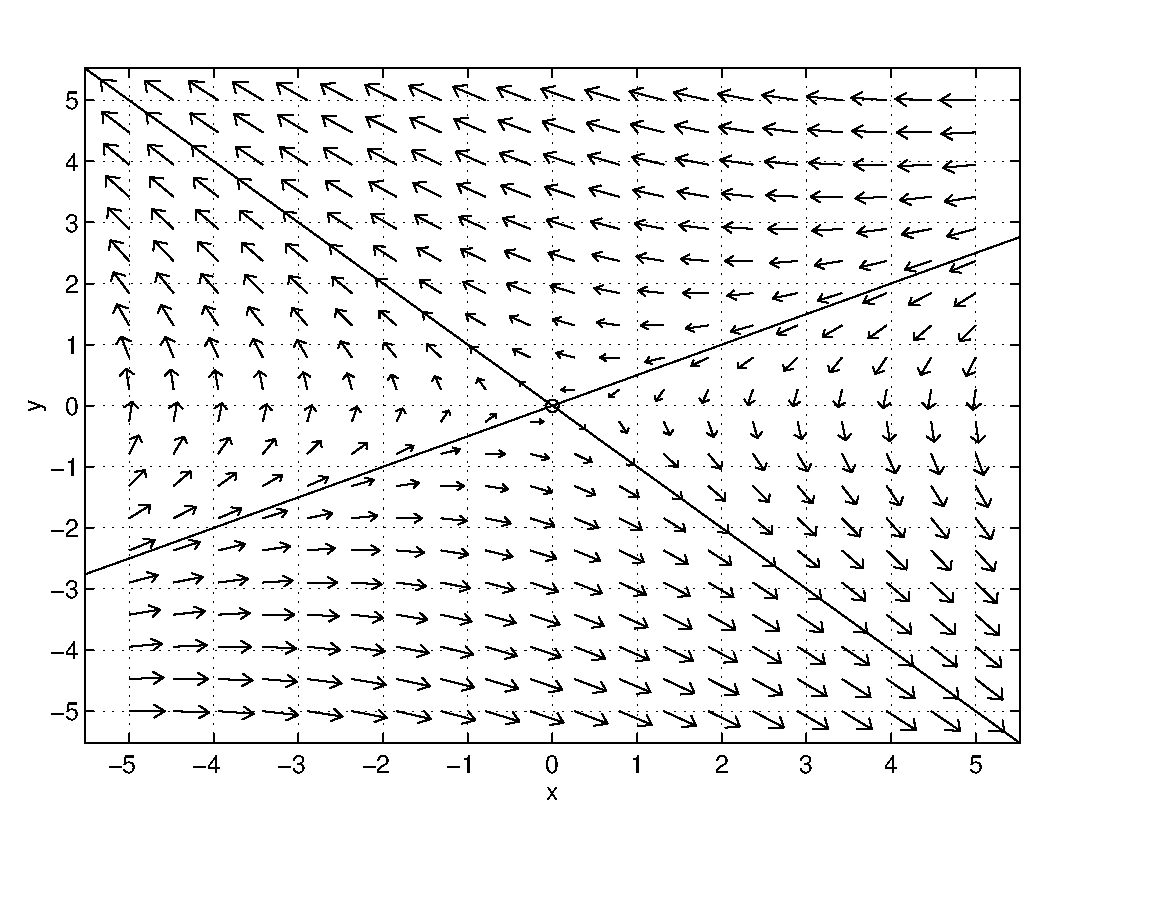
\psfig{file=exfigure/6-1-4a.eps,width=1.8in}
                       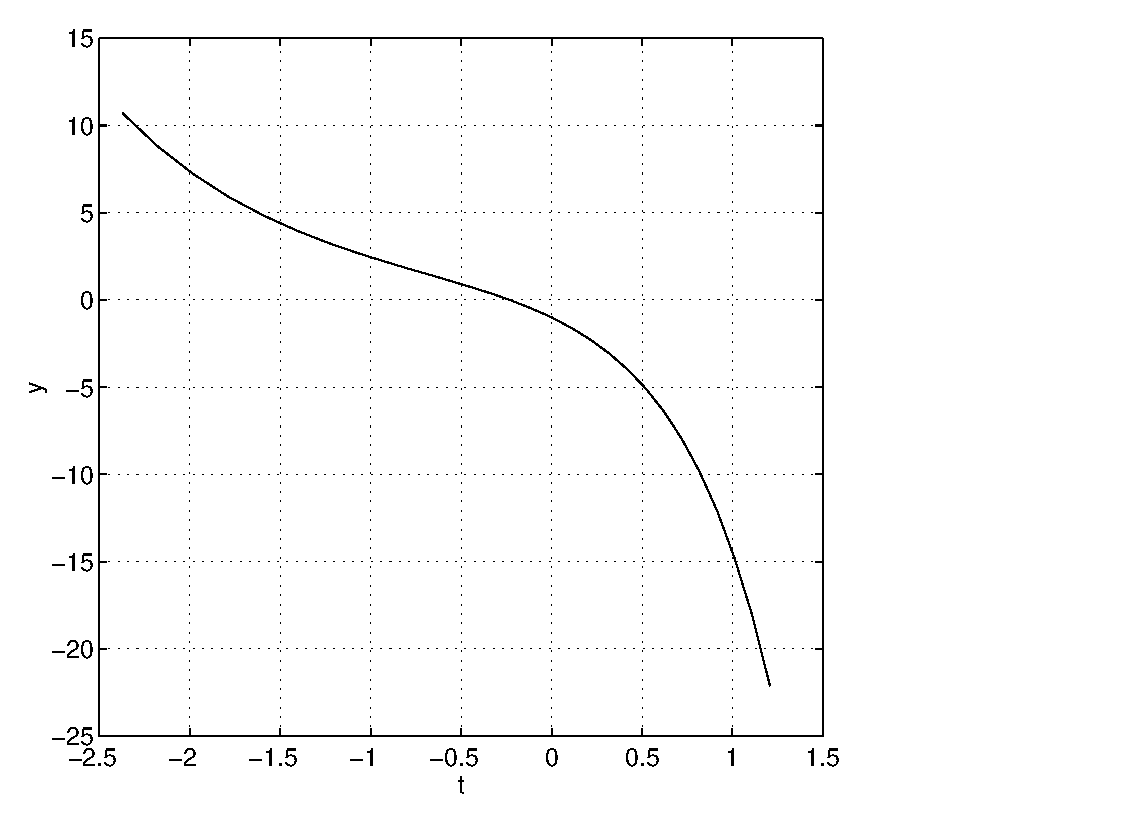
\psfig{file=exfigure/6-1-4b.eps,width=1.8in}
                       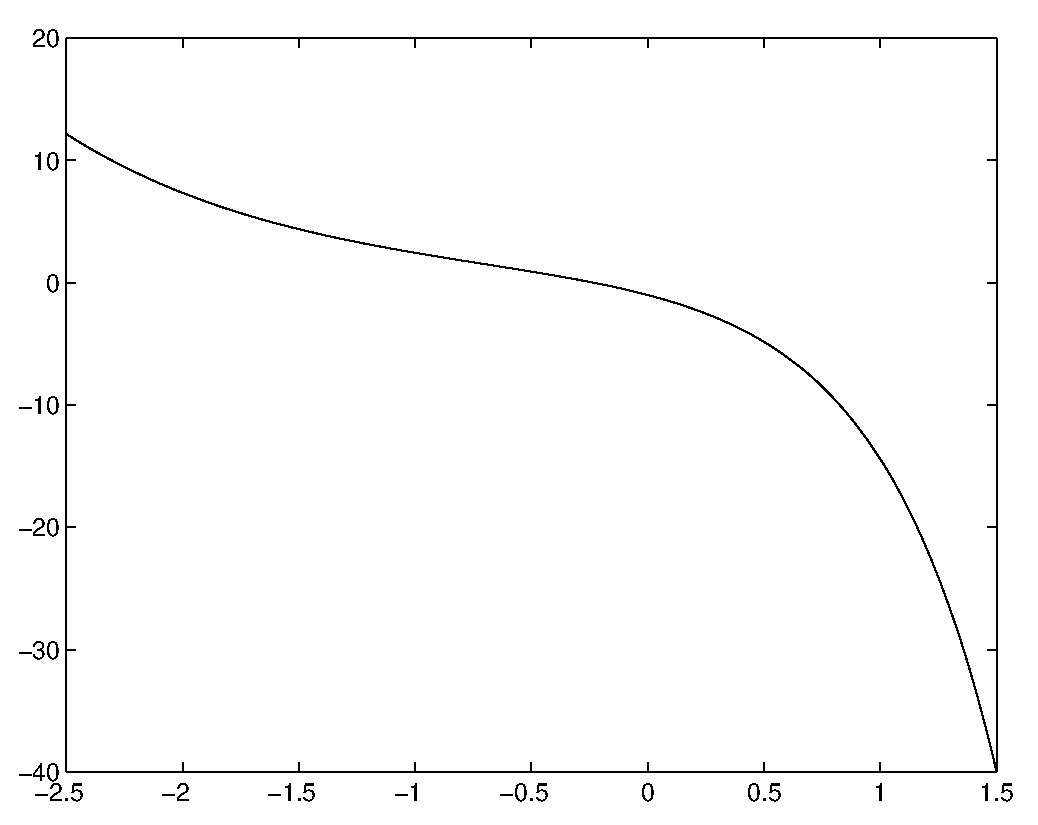
\psfig{file=exfigure/6-1-4c.eps,width=1.8in}}
                \exercapthree{c6.1.4}
\end{figure}




\end{solution}
\end{exercise}




\end{document}
